\documentclass[11pt,journal]{IEEEtran}
%\usepackage{hyperref}
%\usepackage[breaklinks]{hyperref}
\usepackage{breakurl}
\usepackage{url}
\usepackage{listings}
% Set listings to use small monospaced font.
\lstset{basicstyle=\small\ttfamily,tabsize=4}
\usepackage{graphicx}
\ifCLASSOPTIONcompsoc
% IEEE Computer Society needs nocompress option
% requires cite.sty v4.0 or later (November 2003)
\usepackage[nocompress]{cite}

\else
% normal IEEE
\usepackage{cite}
\fi

\hyphenation{op-tical net-works semi-conduc-tor}


\begin{document}
	\title{Exploring the power of the Atelier B automated prover - Interim Report}
	
	\author{Agata~Borkowska,~UID: 1690550,~\IEEEmembership{MSc in Computer Science,~University of Warwick}% <-this % stops a space
		\protect\\
		\thanks{}}
	
	% The paper headers
	
	\markboth{}%
	{ \MakeLowercase{\textit{}}: }
	
	\IEEEcompsoctitleabstractindextext{%
		\begin{abstract}
			%\boldmath
			AtelierB is a tool for formal software development through refinement, using the B-method. It incorporates an automated prover, which has been recognized as the most thorough prover for B set theory, and has been used as a basis for many others. Nevertheless it has multiple shortcomings. Various approaches have been suggested and taken to improve its performance, including extensions to the proof rule base, created by the users. In this work we aim to create such an extension, ensuring that all added rules are sound and well-reasoned. We also aim to identify any limitations of this approach. The secondary goal is to improve the robustness of the software without straying from pure B method, and taking into account the ease of use. As a metric of our success, we use the benchmarks proposed by Conchon and Iguernlala\cite{survey}.
	\end{abstract}
	\begin{IEEEkeywords}
		B method, formal verification
	\end{IEEEkeywords}}
	% IEEEtran.cls defaults to using nonbold math in the Abstract.
	% This preserves the distinction between vectors and scalars. However,
	% if the journal you are submitting to favors bold math in the abstract,
	% then you can use LaTeX's standard command \boldmath at the very start
	% of the abstract to achieve this. Many IEEE journals frown on math
	% in the abstract anyway. In particular, the Computer Society does
	% not want either math or citations to appear in the abstract.
	
	% Note that keywords are not normally used for peerreview papers.
	
	% make the title area
	\maketitle
	
	
	% To allow for easy dual compilation without having to reenter the
	% abstract/keywords data, the \IEEEcompsoctitleabstractindextext text will
	% not be used in maketitle, but will appear (i.e., to be "transported")
	% here as \IEEEdisplaynotcompsoctitleabstractindextext when compsoc mode
	% is not selected <OR> if conference mode is selected - because compsoc
	% conference papers position the abstract like regular (non-compsoc)
	% papers do!
	\IEEEdisplaynotcompsoctitleabstractindextext
	% \IEEEdisplaynotcompsoctitleabstractindextext has no effect when using
	% compsoc under a non-conference mode.
	
	
	% For peer review papers, you can put extra information on the cover
	% page as needed:
	% \ifCLASSOPTIONpeerreview
	% \begin{center} \bfseries EDICS Category: 3-BBND \end{center}
	% \fi
	%
	% For peerreview papers, this IEEEtran command inserts a page break and
	% creates the second title. It will be ignored for other modes.
	\IEEEpeerreviewmaketitle
	
	
	
	\section{Introduction}
	\IEEEPARstart{T}{he} aim of formal specification and verification is to ensure the correctness of software. While overall less popular than quality assurance through testing, it is used in safety-critical areas, such as air traffic control, railway routing, or medical cyber-physical systems, or where testing is too costly or puts the users at risk. It allows for certifying that a given piece of software works as intended, and is error-free.
	
	In some industries, such as railway, it is demanded by the regulations to provide a certificate of correctness for any piece of software. While not required, it is strongly suggested to use formal verification methods, such as B or Z, and indeed they make satisfying the regulations easier.\cite{railway standard}
	
	In this project, we shall focus on the classical B-method, allowing for formal specification through refinement of abstract machines. In the earliest stages of the development process, an abstract machine is defined, which satisfies the requirements and expresses the specification in a more precise and rigorous way. It is a construct based on 1\textsuperscript{st} order logic and set theory. At this point, there is no reasoning about the order of operations and timeline. Additionally the machine may and often will have some nondeterministic elements. The abstract machine then gets refined, the nondeterminism is removed, and the structures and data types become more concrete.
	
	The B-method allows us to do much more than turn an initial specification into an auto-generated code. It gives us a means of documenting the whole software development process, and certifying that the final product indeed meets the requirements.
	
	\subsection{Atelier B tool}
	The tool to support all stages of software development with B-method is Atelier B, created by ClearSy Systems Engineering. In particular it includes a powerful automated prover. We will inspect it and the proof process very closely, as the work in this project is expected to rely on it entirely.
	
	After creating the specification, we can generate proof obligations (POs). They are statements about the consistency of the types of variables, well-defineness and other things that are implied by our definitions or methods. In a correct piece of software, all of the POs should be demonstrated to hold. If there is a PO that cannot be proved to hold by any means, it indicates that there exists an error in the specification.
	
	It is expected that about 75\% of the POs will be demonstrated automatically, and only 5\% of them will require more than 10 s (i.e. proof force 1 or higher)\cite{Prover guide}. The remaining POs will need user input to be discharged. This is done through the automated prover, with the user chosing which rule or tactic to apply, simplifying the hypothesis and in general nudging the prover and pointing it in the right direction.

	\subsection{Shortcomings of Atelier B}
	
	Atelier B is not a perfect tool and the user experience leaves much to be desired. Leuschel \emph{et al.}\cite{San Juan metro} were very critical about it, and it is worth looking closely at the issues they have raised. Their main problem with the tool and the focus of their paper was lack of optimisation, which is not as relevant for us, however they listed others as well. They noted that in the case of undischarged POs, it was "difficult to find out why the proof has failed". This is in line with our own experience.
	
	We will not go into the details of bugs raised in the paper, as the authors have been using Atelier B version 3.6.2, while the one we use 4.2.1, released in December 2014. According to the release notes, more than 150 bugs have been fixed since the previous version. However, no list of known bugs and issues has been found for the newest version\cite{release notes}. Several attempts to gain access to the most up--to-date list of known issues and bug reports for Atelier B have been made. Unfortunately, ClearSy is not responsive, and we have been waiting for five months without success to get their administrator's approval, despite the description on their website stating that the reports are publicly available.
	
	Another issue is mentioned by Medeiros and D\'{e}harbe\cite{BEval}. They point out that Atelier B is falling behind the developments made by researchers in the area of automated theorem proving. It is unsurprising, as the tool's development process is slow due to the need for certification of every update, without which it could not be used in an industrial setting.
	
	While we will not aim to fix these issues, it is necessary for us to be aware of them. It should also be pointed out that despite all its shortcomings, Atelier B is the most popular and the best developed tool. It has been around for over 20 years, and has the largest user base out of all software for development in B. 
	
	\section{Project Aims Restated}
	In this project we shall focus on the Atelier B automated prover, without creating or using any plugins or extensions. The key aim of the project is to see if it is possible to achieve a better ratio of automatically discharged proof obligations by expressing the design requirements in different ways, and if so, we aim to discover general patterns and trends, which we will consolidate into guidelines for other users.
	
	The project is directed at new users of Atelier B, including students and academics who use the tool to study formal methods of development. In our own as well as fellow students' experience, the tool often displays non-intuitive behaviour. The difficulty to understand why a proof has failed was brought up by Leuschel \emph{et al.} in their broad case study\cite{San Juan metro}, among others. We aim to aid the users by providing tips on how to overcome the problems arising from the tool rather than their reasoning.
	
	We have found very scarce advice on how to get started with formal development using Atelier B, especially in terms of practical advice. The majority of the literature concerns examples of large-scale industry projects, which are not helpful for beginners due to their vastness, or very particular topics, such as verifying user-created rules with deep embedding\cite{embedding and theorem proving} or satisfiability modulo theory solvers\cite{SMT}. However we found nothing suggesting at what point adding user-written rules is advised or similar practical guidelines. There is little to nothing bridging the gap between the user manuals and the advanced applications.
	
	The key learning outcome of the project is a deeper understanding of the behaviour of the interactive prover, which is often non-intuitive to the users. We hope that the outcome of this project will help future students and other people hoping to understand the workings of Atelier B's automated prover. The deliverables will include the example scenarios, each one with a full explanation in a more human-friendly manner, the guidelines we have collected over the course of the project, and any additional proof rules together with their proofs.
	
	It is expected that over the course of this project, new questions and ideas will arise. Some, but not all may be pursued, while others will be identified as areas for further research.
	
	Finally, we will not evaluate plugins and extensions to Atelier B, which we have considered doing in the research proposal. In the light of the restated project aims, it does not seem as relevant. New users are unlikely to use them, and we do not want to spread our resources too thinly or rush other, more useful parts of the project.

		
	\section{Methodology}
	\subsection{Overview of the approach}

	We will use multiple scenarios to test the interactive prover. They will be of varied complexity, and demonstrate different aspects of the B method. We will begin with simplest and quite generic scenarios, and increase their complexity to establish at what point the POs stop being discharged automatically, and then proceed until the interactive prover is not sufficient either. 
	
	Nevertheless the method applied to each scenario will follow the same steps. We will begin by using the interactive prover to demonstrate the undischarged proof obligation. It allows us to apply the proof rules of our choice, refine the hypothesis, and otherwise guide the proof.
	
	The next step is to rewrite the problematic expressions in the machines in a way such that they retain their meaning, but are more prover-friendly, and again use the interactive prover. This is the step which was sufficient to fully automatically prove the Bag machine variants discussed later.
	
	If that is still not enough, we will inspect the tactics included in the prover, that is the order in which the proof rule base is searched through and applied. Only if making changes to the tactics is still not enough, we will consider writing our own rules.
	
	The proof rule base is large, but nevertheless finite, and cannot be expected to include every rule a user may need. Still, it is strongly advised by the manuals as well as common to not include user-written rules in the projects, unless it is absolutely necessary. Every such rule has to be rigorously proven. Thus this is the very last step in our method, and so far we have not had the need to use it. 
	
	If we find it necessary to write new rules, we will include them and their proofs with the guidelines and observations, so that others may benefit from them.
	
	We will pay very close attention to what sort of proof obligations are not discharging, and look for similarities between them. For example, are they concerned with well-definedness or rewrite rules? Do they have some other traits, such as types in common? Finally, are there any seemingly simple POs that require a large number of steps in the prover?

	
	It should also be pointed out that the Atelier B Maintenance edition includes a tool for validating mathematical rules. Unfortunately we are unable to gain access to it. It is not a great loss however, as in this project we will focus on other aspects of the tool as well as the proof rule base, and additionally there are almost no references to the tool that assess its usefulness.
	
	
	
	
	\subsection{Choice of Scenarios}
	To recognize the most common problems, we will create a variety of scenarios which are simple and easy to reason about without employing the prover. The scenarios will each focus on a different, but common programming problem, which new users are likely to come across. Examples include formally describing a collection or a graph, and operations on them. 
	
	Such scenarios are exemplary of what beginners might tackle and should prove effective in identifying the most prevalent issues, be it with the implementation of the B-method in the tool or with expressing design requirements formally.
	
	It should also be noted that there is a large difference between the standalone machines we use and the large-scale industry projects. A single machine may result in a dozen proof obligations, while the whole projects end up generating over a thousand. It would be infeasible to use the latter to explore the most basic, underlying problems. On the other had there is a noticeable trend that the expressions in the large projects are kept as simple as possible, and more complicated structures such as sequences are avoided, and hence the problems illustrated by the small machines will be still applicable.
	
	Thus we will keep the scenarios small, but use primarily the same data structures and types as in large projects, hence working on something useful and applicable, but at the same time possible to reason about even without the prover. The latter is key to understanding the behaviour of the interactive prover.

	
	\section{Progress}
	\subsection{Preliminary observations}
	The version of the Atelier B tool used is 4.2.1, with the GUI Version V4.0-50720. It is the freeware version, used commonly for teaching and learning purposes, and available in English from the ClearSy Ltd. website. It is possible although unlikely that over the course of the project it will be updated. If it happens, we will switch to the newer version if it includes only bug fixes or other changes which do not affect the work performed thus far. Otherwise, depending on the extent of the changes, we will either continue using the initial version or switch to the new one, noting any discrepancies.
	
	It is important to understand that the prover can only generate proof obligations and demonstrate that they are satisfied, but is incapable of proving that they are not - this problem is undecidable. In other words, each proof obligation can only be proved or unproved, and the latter can happen for one of two reasons. It is quite likely that a PO is true, but the program cannot prove it automatically because of its complexity. However, the unproved obligations also include the ones that are false and point to errors in the specification. 
	
	Due to their abstract nature, the initial stages of the development are more difficult to reason about and to prove their correctness. The proofs even with the help of the interactive prover become labourious. At the same time there majority of the documentation focuses on the later stages, which is an inconvenience. 
	
	\subsection{The Bag machine}
	The first scenario we have explored is a collection of elements from a given set, with a limit on the number of items it contains. It can be thought of a bag containing at most \texttt{max\_elem} elements from a set of \texttt{ITEMS}. The machine ensures that the limit on the number of elements is not exceeded, and includes operations to add, remove, and query the content of the bag. The most basic form of this machine can be found in Appendix A. 
	
	We have created twelve variations of this machine, exploring different ways of defining the set of items to choose from and the content of the bag. The possibilities for the former include deferred set (a set which is defined at a later stage of the development), enumerated set, or a set of integers. The latter can be expressed as a set or as a mapping of items to the number of each one the bag contains, mindful of the differences in the functionality that it would entail. 
	
	The number of possibilities is of course finite, but going through all of them is a labourous process. Some have resulted in the exact same behaviour (namely a deferred specified in the \texttt{SETS} clause and a set passed as a machine parameter). Others have indicated the underlying implementation of the B-method, not thoroughly documented. 
	
	This simple scenario has already given us insights into how the interactive prover operates. It led to the discovery of the non-commutativity of the logical clauses in the \texttt{INVARIANT} and to understanding of how enumerated sets are implemented. 
	
	Furthermore it allowed us to come with a general method of tackling frustrating proof obligations. In many cases including the goal given by the prover in the \texttt{INVARIANT} clause or the precondition of an operation will result in the proof obligations discharging automatically or even fewer being generated. Whether it is a sound approach, depends on the particular situation. It is likely to be acceptable, as by definition the behaviour of the abstract machine in states not specified in the precondition is nondeterministic. Similarly adding the clause to the \texttt{INVARIANT} may exclude certain states, but these states may not be desired, and thus it attracts the user's attention to the correctness of the specification.
	
	Finally, we have observed that Atelier B displays some undesired behaviour, such as aggressive caching. It is often necessary to force the software to regenerate proof obligations twice after making a change to a machine. Otherwise the resultant proof obligations do not reflect the changes.
	
	
	\subsection{Discrepancies between the B-method and its implementation}
	The B method is well-defined in terms of 1\textsuperscript{st} order logic and set theory. We use Schneider's \emph{The B-Method}\cite{b-method} and Abrial's \emph{The B-book}\cite{b-book} as the main references. However the implementation of it the Atelier B tool does not capture all the nuances and imposes restriction. An example of a discrepancy between the theory and the implementation which we have discovered earlier, is the fact that conjunctions in machine clauses such as the \texttt{INVARIANT} are not commutative, as the rules of logic suggest. To illustrate this, we compare two ways of establishing the bound on a cardinality of a set. According to the Atelier B documentation, the expression \texttt{card(set)} is meaningful only if the set is finite. Thus the following clauses in the \texttt{INVARIANT} do not lead to an undischarged proof obligation:
	
	\begin{lstlisting}
	set : FIN(set) & 
	card(set) <= max_card 
	\end{lstlisting}
	
	However reversing the order of the clauses leads to a proof obligation which cannot be demonstrated automatically or interactively within the prover, related to the finiteness of the set. 
	
	We can only speculate how these discrepancies arose, since the tool is closed-source. In the above example, it is plausible that checking all permutations of the clauses by the automatic prover would be too costly. It is exactly problems such as this one, which can be very frustrating to new users. They can spend a lot of time looking for this simple, but not an obvious solution, and it is tips like this which we would like to collect and present to the those beginning their work with Atelier B.
	
	\subsection{Analysis of the Documentation of Atelier B}
	ClearSy has included multiple guides and manuals with the software. The core documents provided by ClearSy are: 
	\begin{itemize}
		\item \emph{Atelier B 4.0 User Manual}\cite{user manual}
		\item \emph{B Language Reference Manual}\cite{b reference}
		\item \emph{Proof Obligation Manual}\cite{PO reference}
		\item \emph{Interactive Prover Reference Manual}\cite{Prover guide}
	\end{itemize}
	The documentation is voluminous, however redundant or oddly phrased at times and difficult to navigate. An illustrative example is the case of an enumerated set. We have included it in one of the variations of the Bag machine and obtained multiple undischarged proof obligations, imposing restrictions on the range and domain of a set. We have found little on how the enumerated sets are implemented, and we have come across the following cryptic description in the \emph{Interactive Prover Reference Manual}: "Every enumerated set is defined as the set comprising all of its elements, and the elements are distinct two by two." It is now understood as enumerated sets being mappings from an interval of integers, beginning at 1, to the items listed. This was discovered by close observation of the proof obligations generated, and confirmed by an example listed in \emph{Interactive Prover Reference Manual}. It is worth mentioning that this example was not related to the current problem and was accompanied by scarce explanation. It serves well to show how tedious cross-checking the manuals is.

	They were all initially written in French and translated to English. The translation was not thorough, and especially examples remained in the original language, which makes them more difficult to follow.
	
	Other documents, such as \emph{Redaction Guide for Mathematical Rules}\cite{Redacting rules}, have been translated by academics, without an endorsement from ClearSy Ltd. Nevertheless they are important and immensely relevant to the project.
	
	This example raises a question of how many more documents we are unaware of, because they have not been translated. It is unfortunate that the original documents are of little use to us, given the lack of fluency in French. On the other hand they are inaccessible to most students and academics who may wish to use Atelier B. Thus we will not rely on the non-English documents, while being mindful of the fact that they exist and may contain useful information.

	
	\section{Future work}
	\subsection{Scenarios to explore}
	The work on the variations of the Bag machine has been concluded and we are able to move onto another scenario. Our choice is another versatile example, namely implementations of a graph. There are multiple ways to describe a graph mathematically - an adjacency matrix, a pair of sets of vertices and edges, etc. To avoid repetition of the work done on the Bag machine, we will use the tips and tricks discovered previously to minimise the number of undischarged proof obligations from the start. Instead we would like to concentrate on proof obligations related to operations and connections between variables.
	
	The graph scenario can be further explored by imposing properties on the graphs. Making the graphs acyclic, connected, or directed will result in more intricate relations between the structures in the abstract machine, and hence hopefully more insightful problems.
	
	Using other scenarios will depend on how effective the graph machine will be. Given that it allows for more variations than an implementation of a set or collection, it may exhaust the data types and structures in the B-method.
	
	In the original project timetable we expected to spend the later part of the project, evaluating plugins and extensions to Atelier B. However, having restated the project aims to focus on the software on its own, we will concentrate on thoroughly and exhaustively analysing the interactive prover with the help of additional scenarios.
	
	Time permitting, we may look at simple refinements of the previously used scenarios, and various ways of structuring.
	
	\subsection{Benchmarking}
	
	As quoted before, it is expected that three quarters of the proof obligations will be discharged automatically\cite{Prover guide}. To be able to compare the rate of discharged proof obligations, we will need to write or otherwise obtain larger machines, which result in a more significant number of proof obligations. That is expected  to take up the last couple of weeks of the project, as intended in the original timetable.

	
	\section{Concluding remarks}
	We have decided to dedicate more time to the exploration of the prover and the analysis of exemplar scenarios than initially planned, rather than spread our resources thinly on evaluating third party software on top of this.	We now plan to methodically and exhaustively analyse scenarios, which we create to demonstrate different aspects of the abstract machines in the B method.  
	
	We needed to spend more time than expected on familiarising ourselves with the Atelier B software, but we have caught up with the original timetable, and the time was definitely well spent. The work done on the Bag machine had firstly helped us find a method to analysing the scenarios. It has then resulted in multiple tips which we hope to pass on to fellow students and academics who struggle to understand the behaviour of the prover. The work has accelerated, thanks to clarifying the aims of the project.
	
	We hope that by the end of the project, we will obtain a sizeable collection of guidelines, thanks to which new users will be able to focus on the problems they are trying to solve rather than the intricacies of the software.
	

	% you can choose not to have a title for an appendix
	% if you want by leaving the argument blank

	
	\IEEEPARstart{}{} 
	
	\begin{thebibliography}{1}
		\bibitem{survey}
		S.~Conchon and M.~ Iguernlala, "Increasing Proofs Automation Rate of Atelier-B Thanks to Alt-Ergo" in \emph{Proc.~1st Int.~Conf.~Reliability, Safety and Security of Railway Systems}. Paris, France, 2016, pp.~243-253
		
		\bibitem{railway standard}
		\emph{Railway applications - Communication, signalling and processing systems}, EN 50128, 2011
		
		\bibitem{release notes}
		\emph{Atelier B version 4.2 release notes}, ClearSy Sys. Eng., Aix-en-Provence, France, 2014
		
		\bibitem{b-method}
		S.~Schneider, \emph{The B-Method: an Introduction}, Basinstoke, Palgrave, c2001
		
		\bibitem{b-book}
		J.-R. Abrial, \emph{The B-book: assigning programs to meanings}, Cambridge, Cambridge Univ. Press, 1996
		
		\bibitem{user manual}
		\emph{Atelier B User Manual}, v.~4.0, ClearSy Sys.~Eng., Aix-en-Provence, France
		
		\bibitem{b reference}
		\emph{B Language Reference Manual}, v.~1.8.7, ClearSy Sys.~Eng., Aix-en-Provence, France
		
		\bibitem{PO reference}
		\emph{Proof Obligations Reference Manual}, v.~3.7, ClearSy Sys.~Eng., Aix-en-Provence, France
		
		\bibitem{Prover guide}
		\emph{Interactive Prover User Manual}, v.~4.0, ClearSy Sys.~Eng., Aix-en-Provence, France
		
		\bibitem{Redacting rules}
		\emph{Redaction guide for mathematical rules} v.~1.1, ClearSy Sys.Ęng., Aix-en-Provence, France, accessible: \url{http://www.atelierb.eu/wp-content/uploads/sites/3/manuels/guide-de-redaction-de-regles-mathematiques-fr.pdf}\\
		Translated by D.~D\'{e}harbe, accessible: 
		\url{http://www.math.pku.edu.cn/teachers/qiuzy/fm_B/Atelier_B/Writing_mathematical_rules.pdf}
		
		\bibitem{embedding and theorem proving}
		M. Jacquel et al., "Verifying B Proof Rules Using Deep Embedding and Automated Theorem Proving" in \emph{Proc. 9th Int. Conf. Software Eng. Formal Methods}, Montevideo, Urugway, Nov. 2011, pp. 253-268
		
		\bibitem{SMT}
		D. D\'{e}harbe, "Integration of SMT-solvers in B and Event-B development environments" in \emph{Sci. Comp. Prog.} vol. 78, Elsevier, March 2013, pp. 310-326
		
		\bibitem{San Juan metro}
		M. Leuschel et al., "Automated property verification for large scale B models with ProB" in \emph{Proc. 2nd Int. Symp. Formal Methods}, Eindhoven, The Netherlands. 2009, pp.~708-723
		
		\bibitem{BEval}
		V. Medeiros Jr. and D. D\'{e}harbe, "BEval: A Plug-in to Extend Atelier B with Current Verification Technologies" in \emph{Proc. 1st Latin Amer. Workshop Formal Methods}, Buenos Aires, Argentina, 20014, pp. 53-58
		

		
	\end{thebibliography}

	\onecolumn
	\appendices
	\section{The Bag machine}
	\begin{lstlisting}
/* Bagmch
 * Author: Agata Borkowska
 * UID: 1690550
 * Creation date: 18/02/2017
 */

/* The simplest version of the bag example */
MACHINE
Bagmch
SETS
	// possible items we can put in the bag
	ITEMS
CONSTANTS
	// max number of items that fit in the bag
	max_elem
PROPERTIES
	max_elem = 3
VARIABLES
	// contents of the bag
	content
INVARIANT
	content <: ITEMS & // it's a subset of ITEMS
	content : FIN(content) & // it's a finite set
	card(content) <= max_elem // it has at most max_elem elements
INITIALISATION
	content := {} // we start with an empty bag
OPERATIONS
	/* Adds item aa to the bag, if there's space for it*/
	additem(aa) =
	PRE
		aa : ITEMS
	THEN
		IF
			// only add item if we won't exceed the limit
			card(content) < max_elem
		THEN
			content := content \/ {aa}
		END
	END;
	
	/* removes aa from the bag (does nothing if aa not in the bag) */
	removeitem(aa) =
	PRE
		aa : ITEMS
	THEN
		content := content - {aa}
	END;
	
	/* getter for the content*/
	items <-- getcontents = items := content;
	
	/* query how many items are in the bag */
	nn <-- howmany = nn := card(content);
	
	/* checks if the item aa is in the bag */
	check <-- isin(aa) = 
	PRE
		aa : ITEMS
	THEN
		IF 
			aa : content
		THEN
			check := TRUE
		ELSE
			check := FALSE
		END
	END
END
\end{lstlisting}

\section{The original Project Timetable}
	\begin{figure*}[here]
	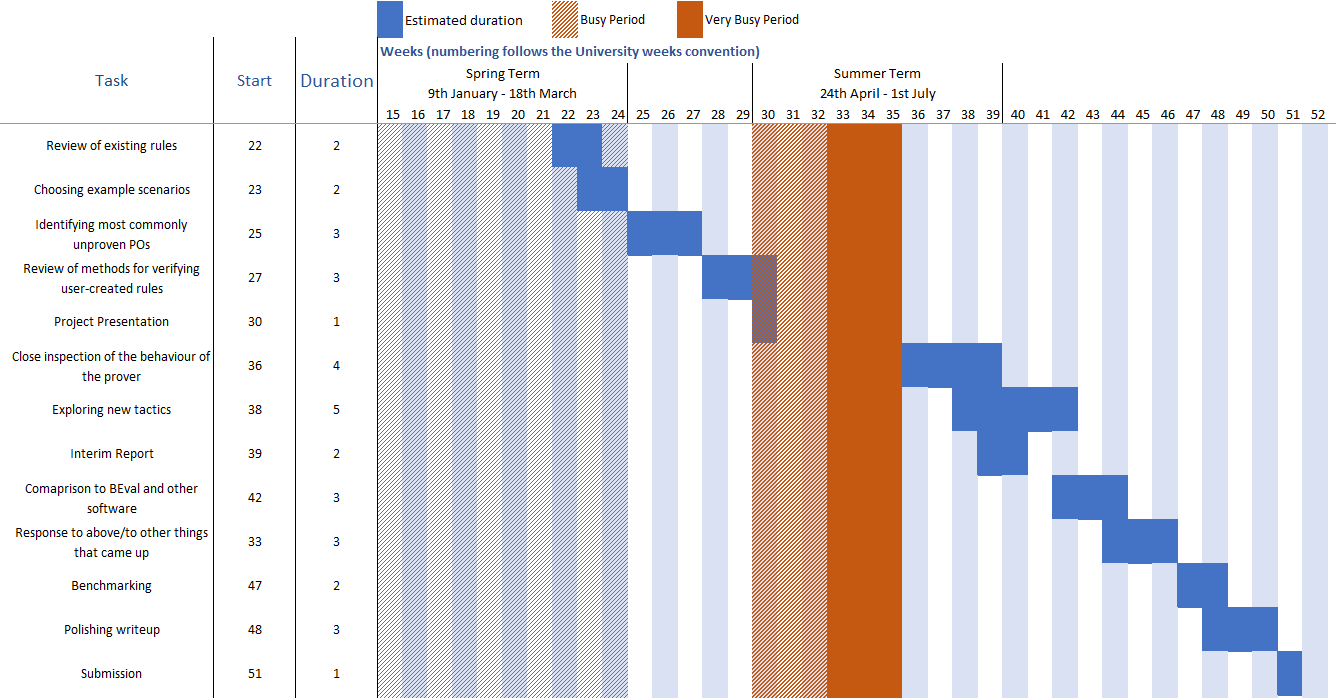
\includegraphics[width=\textwidth]{gantt_chart.png}
	\caption{Gantt chart with the rough timeline of the project}
\end{figure*}
	
	% that's all folks
\end{document}

